\documentclass{templateNote}

\begin{document}

\imagenlogoU{img/LogoElNube.png}
\linklogoU{https://github.com/MarceloPazPezo}
\linkQRDoc{https://github.com/MarceloPazPezo/MyRepo/tree/main/Icinf}
\titulo{PL/SQL: Oracle Express Edition}
\asignatura{Administración y Programación de Base de Datos}
\autor{
    Marcelo Paz
}
\vDoc{1.0.0}

% Metadatos del PDF
\title{[\asignatura]-\titulo}
\author{
    \autor
}
\portada
\margenes % Crear márgenes

\section{Anotaciones}

\subsection{Crear otro usuario para la base de datos}

\begin{enumerate}
    \item Lo primero es permitir el uso de scripts en la sesión actual.
    \begin{figure}[H]
        \centering
        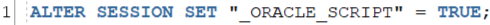
\includegraphics[width=0.5\textwidth]{img/image1.png}
    \end{figure}

    \item Luego en la conexión buscamos el directorio “Otros Usuarios”, le damos clic derecho y luego a “Crear Usuario…”.
    \begin{figure}[H]
        \centering
        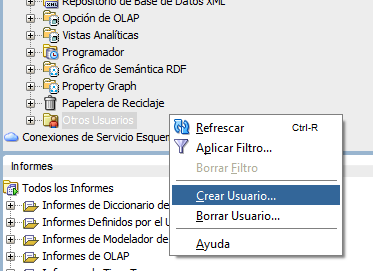
\includegraphics[width=0.5\textwidth]{img/image2.png}
    \end{figure}

    \item Le damos un nombre a nuestro nuevo usuario “USUARIOPRUEBA” y creamos una contraseña.
    \begin{figure}[H]
        \centering
        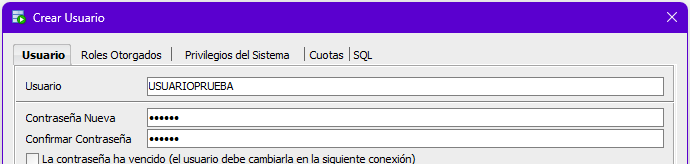
\includegraphics[width=0.8\textwidth]{img/image3.png}
    \end{figure}

    \newpage
    \item Nos vamos a la sección de “Roles Otorgados”, le damos a “CONNECT y DBA” y luego a “Aplicar”.
    \begin{figure}[H]
        \centering
        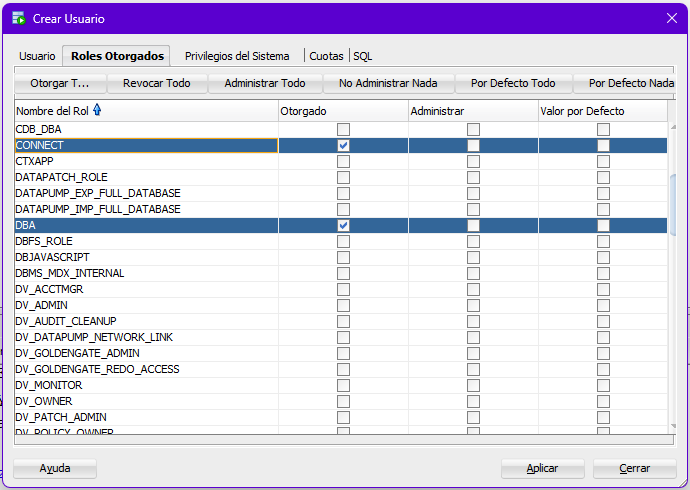
\includegraphics[width=0.7\textwidth]{img/image4.png}
    \end{figure}

    \item Debería aparecernos una ventana para confirmarnos el proceso.
    \begin{figure}[H]
        \centering
        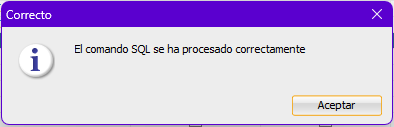
\includegraphics[width=0.5\textwidth]{img/image5.png}
    \end{figure}

    \item Para finalizar al crear una nueva conexión a la BD, debemos ingresar el usuario y darle a “Probar” para validar que la conexión se realiza correctamente (Borde Inferior Izquierdo nos muestra el “Estado: Correcto”).
    \begin{figure}[H]
        \centering
        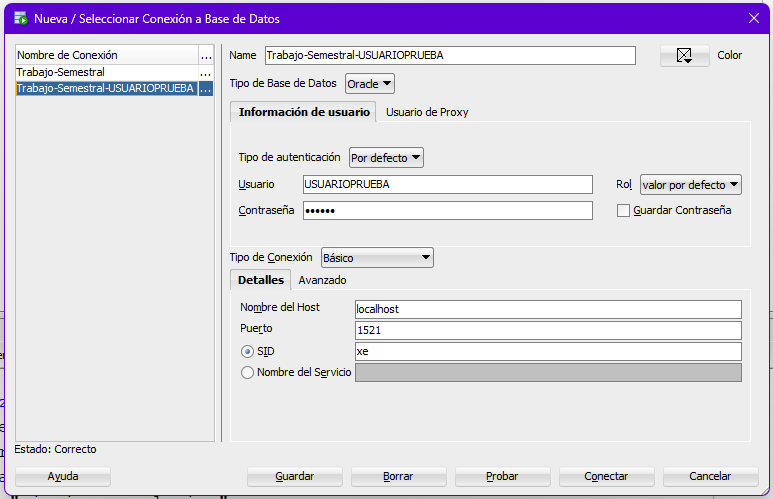
\includegraphics[width=0.7\textwidth]{img/image6.png}
    \end{figure}
\end{enumerate}
\end{document}